En la siguiente sección se podrá observar una breve descripción del modelo de datos a usar. Los autores han decidido usar una base de datos orientada a grafos, Neo4j, por lo cual cada explicación se hará a grandes rasgos sobre un grafo ejemplo generado directamente en Neo4j.

Otro dato a tener en cuenta será que los autores \textbf{sólo describirán el modelo de datos que se ajusta, según ellos, a las funcionalidades a ser implementadas}.

En \cite{anexos_tesis}, el lector podrá encontrar en detalle la descripción de cada nodo etiqueta.

\section{Modelo de datos de gestión de eventos}

Para el prototipo, se ha realizado solamente un evento de práctica deportiva (de carácter libre). El modelo generado se puede apreciar en la figura \ref{fig:modelo_datos_gestion_eventos}.

\begin{figure}[!htb]
  \begin{center}
    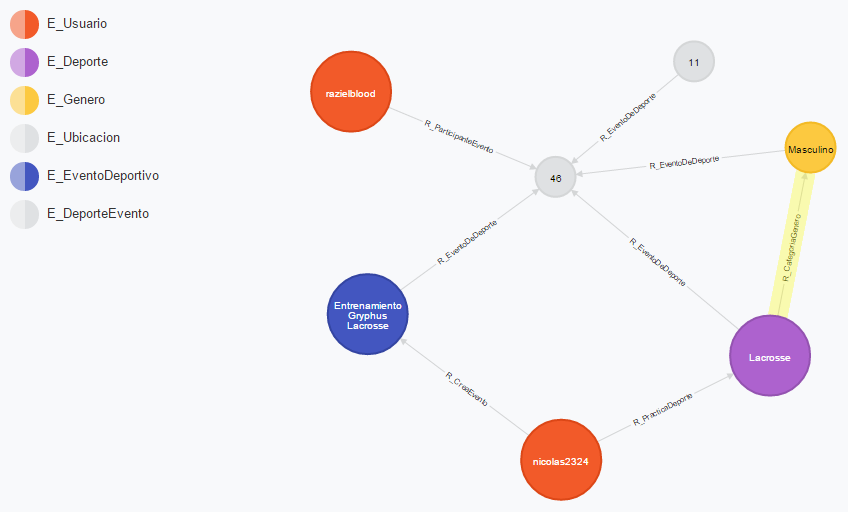
\includegraphics[angle=90,width=9cm,height=15cm]{./imagenes/Modelo_de_datos/Gestion_eventos.png}
    \caption{Modelo de datos de gestión de eventos}
    \label{fig:modelo_datos_gestion_eventos}
    \textbf{Fuente:}  Autores \\
  \end{center}
\end{figure}

Sobre ésta parte del modelo de datos cabe aclarar el papel de la entidad E\_DeporteEvento: Se utilizó un nodo cabecera E\_EventoDeportivo para registrar características generales de un evento; E\_DeporteEvento será la conexión entre un evento deportivo y sus participantes, los deportes que son jugados en dicho evento, las ubicaciones y el genero que jugará en ese evento.

Los nodos que hacen referencia a relaciones n-arias son mostrados en gris.

\section{Modelo de datos de gestión de ubicaciones}

Sobre éste modelo de datos se puede encontrar ubicaciones espaciales atadas a los deportes registrados en la red social. El modelo generado se puede apreciar en la figura \ref{fig:modelo_datos_gestion_ubicaciones}.

\begin{figure}[!htb]
  \begin{center}
    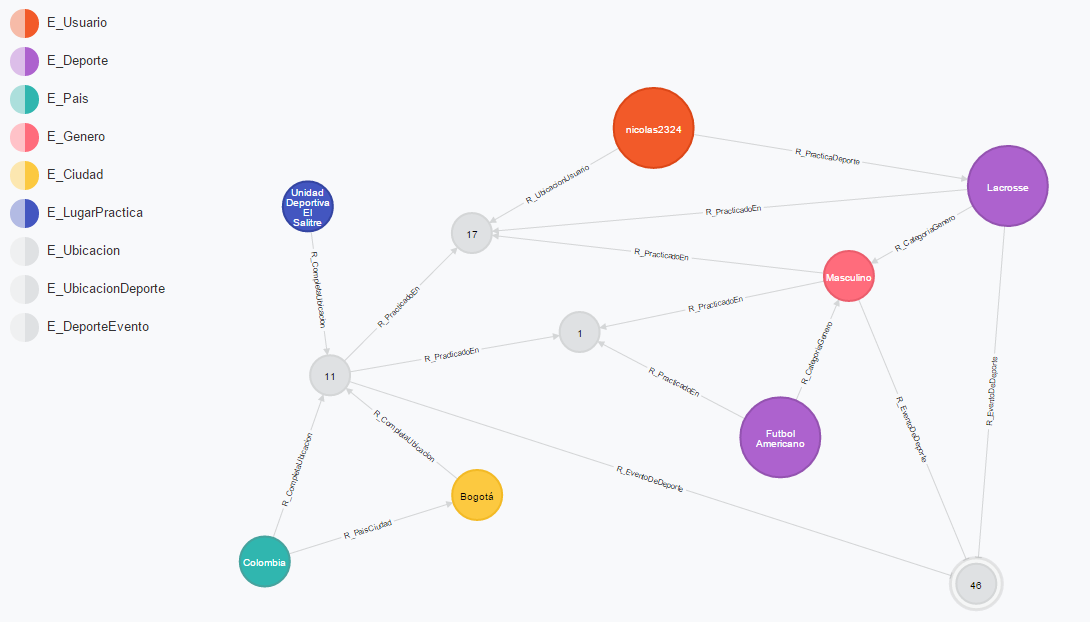
\includegraphics[angle=90,width=9cm,height=15cm]{./imagenes/Modelo_de_datos/Gestion_ubicaciones.png}
    \caption{Modelo de datos de gestión de ubicaciones}
    \label{fig:modelo_datos_gestion_ubicaciones}
    \textbf{Fuente:}  Autores \\
  \end{center}
\end{figure}

Es debido observar los nodos que hacen referencia a relaciones n-arias: uno de ellos se ha llamado E\_UbicacionDeporte, el cual tiene la función de ubicar a un deporte, atado a un respectivo género, en un lugar de práctica; E\_Ubicacion hace un nodo referencia a todos los aspectos de ubicación que tiene una ubicación registrada en la red social, para éste caso, serán los países, ciudades y lugares exactos de práctica del deporte.

Los nodos que hacen referencia a relaciones n-arias son mostrados en gris.

\section{Modelo de datos de gestión de deportes}

Sobre éste modelo de datos se puede apreciar todas las características que los autores han querido atar (para el prototipo) a una entidad deporte, mostrando también su relación con el usuario. La relación con los eventos es debida verla en la figura \ref{fig:modelo_datos_gestion_eventos}, así como la relación en las ubicaciones es debida verla en la figura \ref{fig:modelo_datos_gestion_ubicaciones}. El modelo generado se puede apreciar en la figura \ref{fig:modelo_datos_gestion_deportes}.

\begin{figure}[!htb]
  \begin{center}
    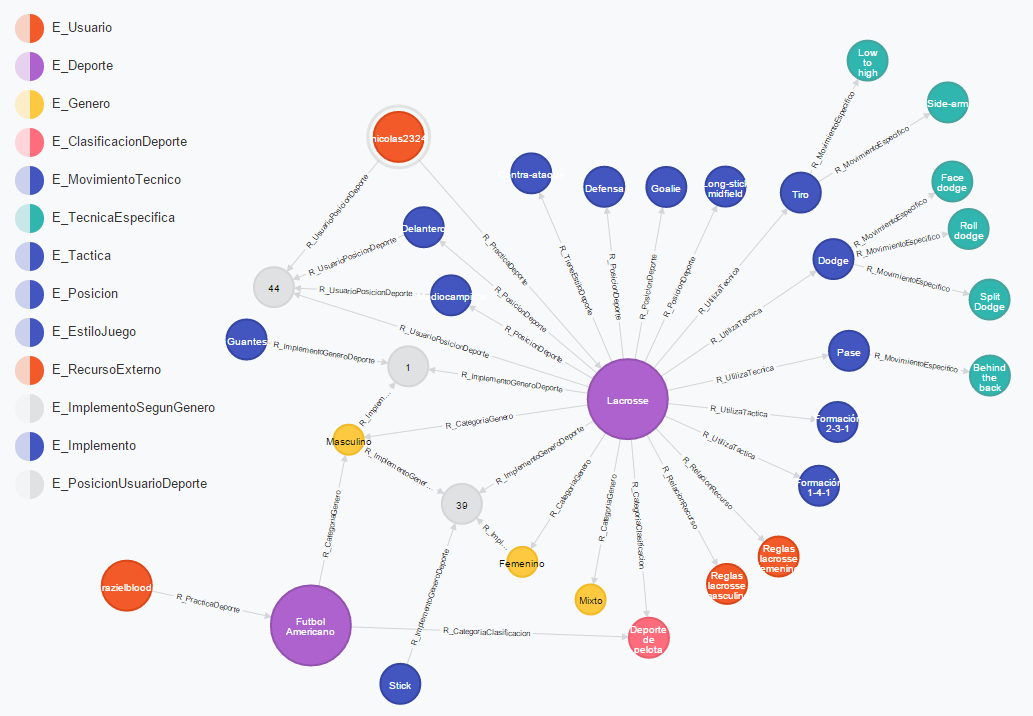
\includegraphics[angle=90,width=11cm,height=15cm]{./imagenes/Modelo_de_datos/Gestion_deportes.png}
    \caption{Modelo de datos de gestión de deportes}
    \label{fig:modelo_datos_gestion_deportes}
    \textbf{Fuente:}  Autores \\
  \end{center}
\end{figure}

Sobre ésta parte del modelo se puede observar cómo todos los elementos que han incluido los autores son elementos unidos como nodos al deporte elegido. Hay dos relaciones n-arias que merecen ser explicadas: La relación n-aria E\_ImplementoSegunGenero es un nodo que actúa como relación n-aria entre E\_Genero, E\_Deporte y E\_Genero, debido a que el equipamiento de un deporte puede variar entre género (por ejemplo, en el lacrosse las mujeres no utilizan guantes protectores); E\_PosicionUsuarioDeporte es un nodo que funciona como relación n-aria entre E\_Deporte, E\_Usuario y E\_Posicion, buscando comunicar en que posiciones juega generalmente un usuario para determinado deporte (en éste caso, el usuario \textit{nicolas2324} juega \textit{lacrosse} en las posiciones \textit{mediocampista} y \textit{delantero}).

Los nodos que hacen referencia a relaciones n-arias son mostrados en gris.

\section{Modelo de datos de gestión de usuarios}

En esta sección del modelo se parametrizan las relaciones básicas de un usuario. Notese que no se incluyen a detalle las relaciones que ya es especificaron en los demás módulos (Multimetdia, por ejemplo), sino os que son inherentes a un uso básico de la aplicación. Se muestra como un usuario puede asumir un rol y puede relacionarse con otros usuarios. La relacion R\_Amigo se muestra en un solo sentido por la limitación de la herramienta que no permite tener relaciones bidireccionales. Se decide dejar una relación en un único sentido por rendimiento. El modelo puede ser apreciado en la figura \ref{fig:modelo_datos_gestion_usuarios}.

\begin{figure}[!htb]
  \begin{center}
    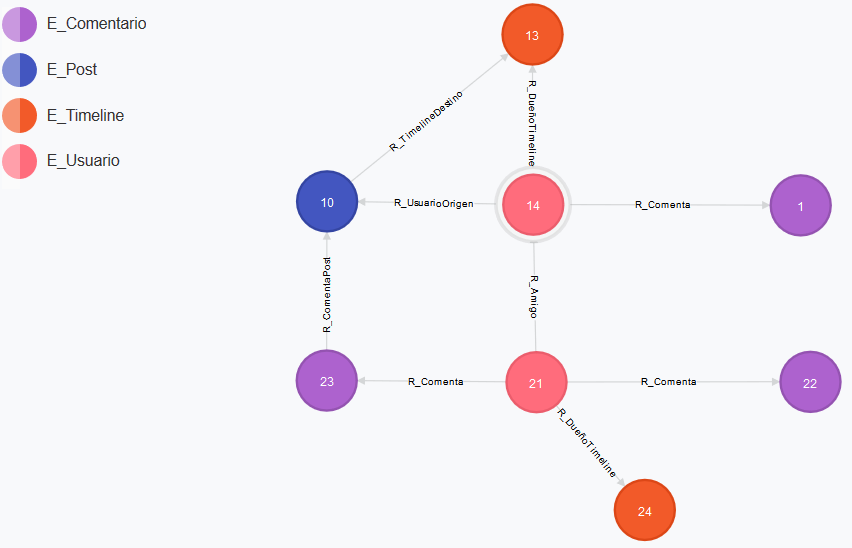
\includegraphics[angle=90,width=9cm,height=15cm]{./imagenes/Modelo_de_datos/Usuarios.png}
    \caption{Modelo de datos de gestión de usuarios}
    \label{fig:modelo_datos_gestion_usuarios}
    \textbf{Fuente:}  Autores \\
  \end{center}
\end{figure}
